% Copyright (c) 2025 Alexander Bluhm <bluhm@genua.de>
%
% Permission to use, copy, modify, and distribute this software for any
% purpose with or without fee is hereby granted, provided that the above
% copyright notice and this permission notice appear in all copies.
%
% THE SOFTWARE IS PROVIDED "AS IS" AND THE AUTHOR DISCLAIMS ALL WARRANTIES
% WITH REGARD TO THIS SOFTWARE INCLUDING ALL IMPLIED WARRANTIES OF
% MERCHANTABILITY AND FITNESS. IN NO EVENT SHALL THE AUTHOR BE LIABLE FOR
% ANY SPECIAL, DIRECT, INDIRECT, OR CONSEQUENTIAL DAMAGES OR ANY DAMAGES
% WHATSOEVER RESULTING FROM LOSS OF USE, DATA OR PROFITS, WHETHER IN AN
% ACTION OF CONTRACT, NEGLIGENCE OR OTHER TORTIOUS ACTION, ARISING OUT OF
% OR IN CONNECTION WITH THE USE OR PERFORMANCE OF THIS SOFTWARE.

\documentclass[14pt,aspectratio=169]{beamer}
\usetheme{Frankfurt}
\usepackage{tikz}
\usepackage{framed}
\usepackage{adjustbox}
\usepackage{graphicx}
\usepackage{varwidth}
\usepackage{tipa}
\usepackage{alltt}
\usepackage{xcolor}
\usepackage{upquote}
\usepackage[T1]{fontenc}
\usepackage{textcomp}
\usetikzlibrary{shapes.arrows}
\usetikzlibrary{shapes.geometric}
\usetikzlibrary{shapes.multipart}
\usetikzlibrary{shapes.symbols}
\author{Alexander Bluhm}
\title{Running TCP Input in Parallel}
\institute{genua GmbH\\ \url{bluhm@genua.de}\\ \url{bluhm@openbsd.org}}
\date{January 2025}
\let\Tiny\tiny

\begin{document}

\begin{frame}
\titlepage
\end{frame}

\section{Packet Queues}
\begin{frame}{Agenda}
\tableofcontents[currentsection]
\end{frame}

\subsection{Input Queues}
\begin{frame}{Input Queues}
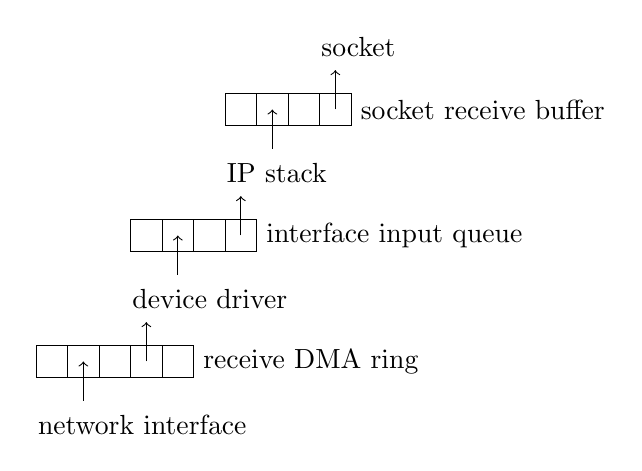
\begin{tikzpicture}
  \draw (0,0)
    node (ni) [right] {network interface} ++(.1,.6)
    rectangle ++(.4,.4) rectangle ++(.4,-.4)
    rectangle ++(.4,.4) rectangle ++(.4,-.4)
    rectangle ++(.4,.4) ++(0,-.2)
    node (rx) [right] {receive DMA ring} ++(-.5-1*.4,.8)
    node (dd) [right] {device driver} ++(.1,.6)
    rectangle ++(.4,.4) rectangle ++(.4,-.4)
    rectangle ++(.4,.4) rectangle ++(.4,-.4) ++(0,.2)
    node (iq) [right] {interface input queue} ++(-.5,.8)
    node (is) [right] {IP stack} ++(.1,.6)
    rectangle ++(.4,.4) rectangle ++(.4,-.4)
    rectangle ++(.4,.4) rectangle ++(.4,-.4) ++(0,.2)
    node (rb) [right] {socket receive buffer} ++(-.5,.8)
    node (so) [right] {socket}
    ;
  \path (node cs:name=ni,anchor=west) +(.3+1*.4,.3) coordinate (nio) {};
  \path (node cs:name=rx,anchor=west) +(-.2-3*.4,0) coordinate (rxi) {};
  \draw[->] (nio) -- (rxi);
  \path (node cs:name=rx,anchor=west) +(-.2-1*.4,0) coordinate (rxo) {};
  \path (node cs:name=dd,anchor=west) +(.3,-.3) coordinate (ddi) {};
  \draw[->] (rxo) -- (ddi);
  \path (node cs:name=dd,anchor=west) +(.3+1*.4,.3) coordinate (ddo) {};
  \path (node cs:name=iq,anchor=west) +(-.2-2*.4,0) coordinate (iqi) {};
  \draw[->] (ddo) -- (iqi);
  \path (node cs:name=iq,anchor=west) +(-.2,0) coordinate (iqo) {};
  \path (node cs:name=is,anchor=west) +(.3,-.3) coordinate (isi) {};
  \draw[->] (iqo) -- (isi);
  \path (node cs:name=is,anchor=west) +(.3+1*.4,.3) coordinate (iso) {};
  \path (node cs:name=rb,anchor=west) +(-.2-2*.4,0) coordinate (rbi) {};
  \draw[->] (iso) -- (rbi);
  \path (node cs:name=rb,anchor=west) +(-.2,0) coordinate (rbo) {};
  \path (node cs:name=so,anchor=west) +(.3,-.3) coordinate (soi) {};
  \draw[->] (rbo) -- (soi);
\end{tikzpicture}
\end{frame}

\subsection{Output Queues}
\begin{frame}{Output Queues}
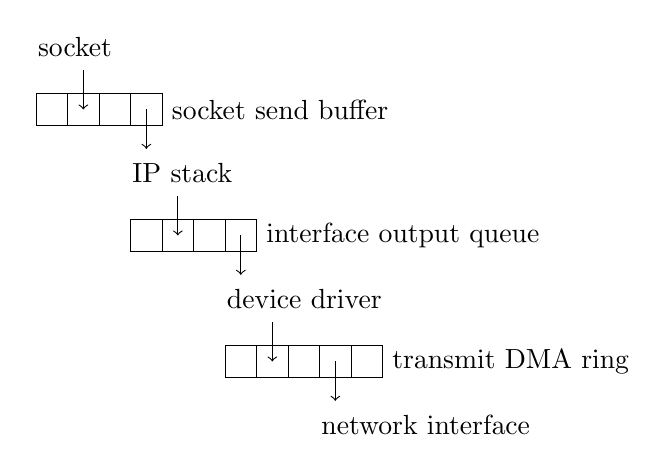
\begin{tikzpicture}
  \draw (0,0)
    node (so) [right] {socket} ++(.1,-.6)
    rectangle ++(.4,-.4) rectangle ++(.4,.4)
    rectangle ++(.4,-.4) rectangle ++(.4,.4) ++(0,-.2)
    node (sb) [right] {socket send buffer} ++(-.5,-.8)
    node (is) [right] {IP stack} ++(.1,-.6)
    rectangle ++(.4,-.4) rectangle ++(.4,.4)
    rectangle ++(.4,-.4) rectangle ++(.4,.4) ++(0,-.2)
    node (oq) [right] {interface output queue} ++(-.5,-.8)
    node (dd) [right] {device driver} ++(.1,-.6)
    rectangle ++(.4,-.4) rectangle ++(.4,.4)
    rectangle ++(.4,-.4) rectangle ++(.4,.4)
    rectangle ++(.4,-.4) ++(0,.2)
    node (tx) [right] {transmit DMA ring} ++(-.5-1*.4,-.8)
    node (ni) [right] {network interface}
    ;
  \path (node cs:name=so,anchor=west) +(.3+1*.4,-.3) coordinate (soo) {};
  \path (node cs:name=sb,anchor=west) +(-.2-2*.4,0) coordinate (sbi) {};
  \draw[->] (soo) -- (sbi);
  \path (node cs:name=sb,anchor=west) +(-.2,0) coordinate (sbo) {};
  \path (node cs:name=is,anchor=west) +(.3,.3) coordinate (isi) {};
  \draw[->] (sbo) -- (isi);
  \path (node cs:name=is,anchor=west) +(.3+1*.4,-.3) coordinate (iso) {};
  \path (node cs:name=oq,anchor=west) +(-.2-2*.4,0) coordinate (oqi) {};
  \draw[->] (iso) -- (oqi);
  \path (node cs:name=oq,anchor=west) +(-.2,0) coordinate (oqo) {};
  \path (node cs:name=dd,anchor=west) +(.3,.3) coordinate (ddi) {};
  \draw[->] (oqo) -- (ddi);
  \path (node cs:name=dd,anchor=west) +(.3+1*.4,-.3) coordinate (ddo) {};
  \path (node cs:name=tx,anchor=west) +(-.2-3*.4,0) coordinate (txi) {};
  \draw[->] (ddo) -- (txi);
  \path (node cs:name=tx,anchor=west) +(-.2-1*.4,0) coordinate (txo) {};
  \path (node cs:name=ni,anchor=west) +(.3,.3) coordinate (nii) {};
  \draw[->] (txo) -- (nii);
\end{tikzpicture}
\end{frame}

\section{IP Stack}
\begin{frame}{Agenda}
\tableofcontents[currentsection]
\end{frame}

\subsection{Protocol Stack}
\begin{frame}{Protocol Stack}
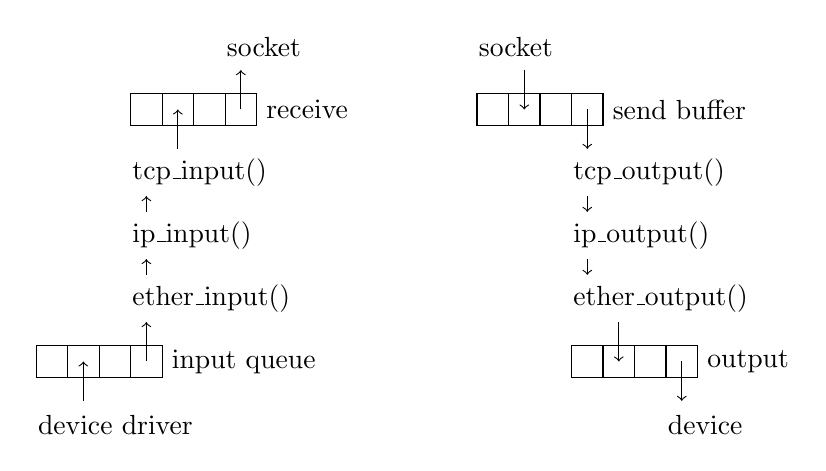
\begin{tikzpicture}
  \draw (0,0)
    node (idd) [right] {device driver} ++(.1,.6)
    rectangle ++(.4,.4) rectangle ++(.4,-.4)
    rectangle ++(.4,.4) rectangle ++(.4,-.4) ++(0,.2)
    node (iq) [right] {input queue} ++(-.5,.8)
    node (ei) [right] {ether\_input()} ++(0,.8)
    node (ii) [right] {ip\_input()} ++(0,.8)
    node (ti) [right] {tcp\_input()} ++(.1,.6)
    rectangle ++(.4,.4) rectangle ++(.4,-.4)
    rectangle ++(.4,.4) rectangle ++(.4,-.4) ++(0,.2)
    node (rb) [right] {receive} ++(-.5,.8)
    node (iso) [right] {socket} ++(3.2,0)

    node (oso) [right] {socket} ++(.1,-.6)
    rectangle ++(.4,-.4) rectangle ++(.4,.4)
    rectangle ++(.4,-.4) rectangle ++(.4,.4) ++(0,-.2)
    node (sb) [right] {send buffer} ++(-.5,-.8)
    node (to) [right] {tcp\_output()} ++(0,-.8)
    node (io) [right] {ip\_output()} ++(0,-.8)
    node (eo) [right] {ether\_output()} ++(.1,-.6)
    rectangle ++(.4,-.4) rectangle ++(.4,.4)
    rectangle ++(.4,-.4) rectangle ++(.4,.4) ++(0,-.2)
    node (oq) [right] {output} ++(-.5,-.8)
    node (odd) [right] {device}
    ;
  \path (node cs:name=idd,anchor=west) +(.3+1*.4,.3) coordinate (iddo) {};
  \path (node cs:name=iq,anchor=west) +(-.2-2*.4,0) coordinate (iqi) {};
  \draw[->] (iddo) -- (iqi);
  \path (node cs:name=iq,anchor=west) +(-.2,0) coordinate (iqo) {};
  \path (node cs:name=ei,anchor=west) +(.3,-.3) coordinate (iei) {};
  \draw[->] (iqo) -- (iei);
  \path (node cs:name=ei,anchor=west) +(.3,.3) coordinate (eio) {};
  \path (node cs:name=ii,anchor=west) +(.3,-.3) coordinate (iii) {};
  \draw[->] (eio) -- (iii);
  \path (node cs:name=ii,anchor=west) +(.3,.3) coordinate (iio) {};
  \path (node cs:name=ti,anchor=west) +(.3,-.3) coordinate (tii) {};
  \draw[->] (iio) -- (tii);
  \path (node cs:name=ti,anchor=west) +(.3+1*.4,.3) coordinate (iti) {};
  \path (node cs:name=rb,anchor=west) +(-.2-2*.4,0) coordinate (rbi) {};
  \draw[->] (iti) -- (rbi);
  \path (node cs:name=rb,anchor=west) +(-.2,0) coordinate (rbo) {};
  \path (node cs:name=iso,anchor=west) +(.3,-.3) coordinate (isoi) {};
  \draw[->] (rbo) -- (isoi);

  \path (node cs:name=oso,anchor=west) +(.3+1*.4,-.3) coordinate (osoo) {};
  \path (node cs:name=sb,anchor=west) +(-.2-2*.4,0) coordinate (sbi) {};
  \draw[->] (osoo) -- (sbi);
  \path (node cs:name=sb,anchor=west) +(-.2,0) coordinate (sbo) {};
  \path (node cs:name=to,anchor=west) +(.3,.3) coordinate (toi) {};
  \draw[->] (sbo) -- (toi);
  \path (node cs:name=to,anchor=west) +(.3,-.3) coordinate (too) {};
  \path (node cs:name=io,anchor=west) +(.3,.3) coordinate (ioi) {};
  \draw[->] (too) -- (ioi);
  \path (node cs:name=io,anchor=west) +(.3,-.3) coordinate (ioo) {};
  \path (node cs:name=eo,anchor=west) +(.3,.3) coordinate (eoi) {};
  \draw[->] (ioo) -- (eoi);
  \path (node cs:name=eo,anchor=west) +(.3+1*.4,-.3) coordinate (eoo) {};
  \path (node cs:name=oq,anchor=west) +(-.2-2*.4,0) coordinate (oqi) {};
  \draw[->] (eoo) -- (oqi);
  \path (node cs:name=oq,anchor=west) +(-.2,0) coordinate (oqo) {};
  \path (node cs:name=odd,anchor=west) +(.3,.3) coordinate (oddi) {};
  \draw[->] (oqo) -- (oddi);
\end{tikzpicture}
\end{frame}

\subsection{IP Forwarding}
\begin{frame}{IP Forwarding}
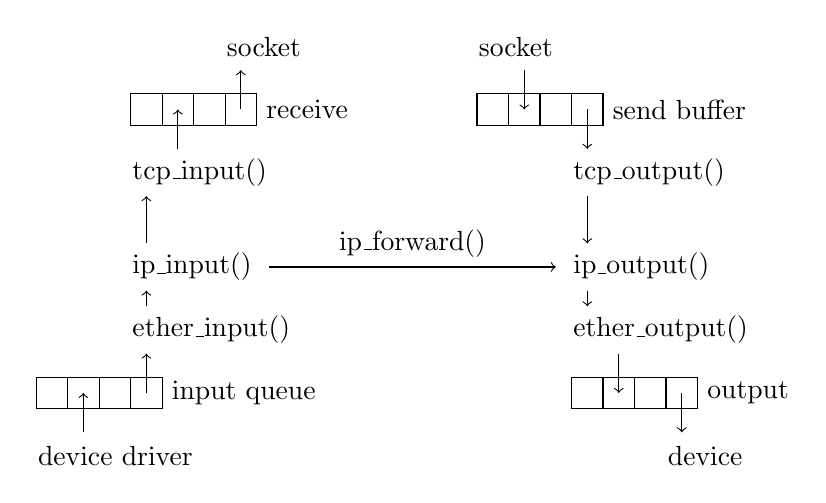
\begin{tikzpicture}
  \draw (0,0)
    node (idd) [right] {device driver} ++(.1,.6)
    rectangle ++(.4,.4) rectangle ++(.4,-.4)
    rectangle ++(.4,.4) rectangle ++(.4,-.4) ++(0,.2)
    node (iq) [right] {input queue} ++(-.5,.8)
    node (ei) [right] {ether\_input()} ++(0,.8)
    node (ii) [right] {ip\_input()} ++(0,1.2)
    node (ti) [right] {tcp\_input()} ++(.1,.6)
    rectangle ++(.4,.4) rectangle ++(.4,-.4)
    rectangle ++(.4,.4) rectangle ++(.4,-.4) ++(0,.2)
    node (rb) [right] {receive} ++(-.5,.8)
    node (iso) [right] {socket} ++(3.2,0)

    node (oso) [right] {socket} ++(.1,-.6)
    rectangle ++(.4,-.4) rectangle ++(.4,.4)
    rectangle ++(.4,-.4) rectangle ++(.4,.4) ++(0,-.2)
    node (sb) [right] {send buffer} ++(-.5,-.8)
    node (to) [right] {tcp\_output()} ++(0,-1.2)
    node (io) [right] {ip\_output()} ++(0,-.8)
    node (eo) [right] {ether\_output()} ++(.1,-.6)
    rectangle ++(.4,-.4) rectangle ++(.4,.4)
    rectangle ++(.4,-.4) rectangle ++(.4,.4) ++(0,-.2)
    node (oq) [right] {output} ++(-.5,-.8)
    node (odd) [right] {device}
    ;
  \path (node cs:name=idd,anchor=west) +(.3+1*.4,.3) coordinate (iddo) {};
  \path (node cs:name=iq,anchor=west) +(-.2-2*.4,0) coordinate (iqi) {};
  \draw[->] (iddo) -- (iqi);
  \path (node cs:name=iq,anchor=west) +(-.2,0) coordinate (iqo) {};
  \path (node cs:name=ei,anchor=west) +(.3,-.3) coordinate (iei) {};
  \draw[->] (iqo) -- (iei);
  \path (node cs:name=ei,anchor=west) +(.3,.3) coordinate (eio) {};
  \path (node cs:name=ii,anchor=west) +(.3,-.3) coordinate (iii) {};
  \draw[->] (eio) -- (iii);
  \path (node cs:name=ii,anchor=west) +(.3,.3) coordinate (iio) {};
  \path (node cs:name=ti,anchor=west) +(.3,-.3) coordinate (tii) {};
  \draw[->] (iio) -- (tii);
  \path (node cs:name=ti,anchor=west) +(.3+1*.4,.3) coordinate (iti) {};
  \path (node cs:name=rb,anchor=west) +(-.2-2*.4,0) coordinate (rbi) {};
  \draw[->] (iti) -- (rbi);
  \path (node cs:name=rb,anchor=west) +(-.2,0) coordinate (rbo) {};
  \path (node cs:name=iso,anchor=west) +(.3,-.3) coordinate (isoi) {};
  \draw[->] (rbo) -- (isoi);

  \path (node cs:name=oso,anchor=west) +(.3+1*.4,-.3) coordinate (osoo) {};
  \path (node cs:name=sb,anchor=west) +(-.2-2*.4,0) coordinate (sbi) {};
  \draw[->] (osoo) -- (sbi);
  \path (node cs:name=sb,anchor=west) +(-.2,0) coordinate (sbo) {};
  \path (node cs:name=to,anchor=west) +(.3,.3) coordinate (toi) {};
  \draw[->] (sbo) -- (toi);
  \path (node cs:name=to,anchor=west) +(.3,-.3) coordinate (too) {};
  \path (node cs:name=io,anchor=west) +(.3,.3) coordinate (ioi) {};
  \draw[->] (too) -- (ioi);
  \path (node cs:name=io,anchor=west) +(.3,-.3) coordinate (ioo) {};
  \path (node cs:name=eo,anchor=west) +(.3,.3) coordinate (eoi) {};
  \draw[->] (ioo) -- (eoi);
  \path (node cs:name=eo,anchor=west) +(.3+1*.4,-.3) coordinate (eoo) {};
  \path (node cs:name=oq,anchor=west) +(-.2-2*.4,0) coordinate (oqi) {};
  \draw[->] (eoo) -- (oqi);
  \path (node cs:name=oq,anchor=west) +(-.2,0) coordinate (oqo) {};
  \path (node cs:name=odd,anchor=west) +(.3,.3) coordinate (oddi) {};
  \draw[->] (oqo) -- (oddi);

  \path (node cs:name=ii,anchor=east) +(.1,0) coordinate (ifo) {};
  \path (node cs:name=io,anchor=west) +(-.1,0) coordinate (ifi) {};
  \draw[->] (ifo) -- (ifi) node [midway,above] {ip\_forward()};
\end{tikzpicture}
\end{frame}

\subsection{UDP}
\begin{frame}{UDP}
\begin{tikzpicture}
  \draw (0,0)
    node (idd) [right] {device driver} ++(.1,.6)
    rectangle ++(.4,.4) rectangle ++(.4,-.4)
    rectangle ++(.4,.4) rectangle ++(.4,-.4) ++(0,.2)
    node (iq) [right] {input queue} ++(-.5,.8)
    node (ei) [right] {ether\_input()} ++(0,.8)
    node (ii) [right] {ip\_input()} ++(0,1.2)
    node (ui) [right] {udp\_input()} ++(.1,.6)
    rectangle ++(.4,.4) rectangle ++(.4,-.4)
    rectangle ++(.4,.4) rectangle ++(.4,-.4) ++(0,.2)
    node (rb) [right] {receive buffer} ++(-.5,.8)
    node (iso) [right] {socket} ++(4.4,0)

    node (oso) [right] {socket} ++(0,-1.6)
    node (uo) [right] {udp\_output()} ++(0,-1.2)
    node (io) [right] {ip\_output()} ++(0,-.8)
    node (eo) [right] {ether\_output()} ++(.1,-.6)
    rectangle ++(.4,-.4) rectangle ++(.4,.4)
    rectangle ++(.4,-.4) rectangle ++(.4,.4) ++(0,-.2)
    node (oq) [right] {output} ++(-.5,-.8)
    node (odd) [right] {device}
    ;
  \path (node cs:name=idd,anchor=west) +(.3+1*.4,.3) coordinate (iddo) {};
  \path (node cs:name=iq,anchor=west) +(-.2-2*.4,0) coordinate (iqi) {};
  \draw[->] (iddo) -- (iqi);
  \path (node cs:name=iq,anchor=west) +(-.2,0) coordinate (iqo) {};
  \path (node cs:name=ei,anchor=west) +(.3,-.3) coordinate (iei) {};
  \draw[->] (iqo) -- (iei);
  \path (node cs:name=ei,anchor=west) +(.3,.3) coordinate (eio) {};
  \path (node cs:name=ii,anchor=west) +(.3,-.3) coordinate (iii) {};
  \draw[->] (eio) -- (iii);
  \path (node cs:name=ii,anchor=west) +(.3,.3) coordinate (iio) {};
  \path (node cs:name=ui,anchor=west) +(.3,-.3) coordinate (uii) {};
  \draw[->] (iio) -- (uii);
  \path (node cs:name=ti,anchor=west) +(.3+1*.4,.3) coordinate (iti) {};
  \path (node cs:name=rb,anchor=west) +(-.2-2*.4,0) coordinate (rbi) {};
  \draw[->] (iti) -- (rbi);
  \path (node cs:name=rb,anchor=west) +(-.2,0) coordinate (rbo) {};
  \path (node cs:name=iso,anchor=west) +(.3,-.3) coordinate (isoi) {};
  \draw[->] (rbo) -- (isoi);

  \path (node cs:name=oso,anchor=west) +(.3,-.3) coordinate (osoo) {};
  \path (node cs:name=uo,anchor=west) +(.3,.3) coordinate (uoi) {};
  \draw[->] (osoo) -- (uoi);
  \path (node cs:name=uo,anchor=west) +(.3,-.3) coordinate (uoo) {};
  \path (node cs:name=io,anchor=west) +(.3,.3) coordinate (ioi) {};
  \draw[->] (uoo) -- (ioi);
  \path (node cs:name=io,anchor=west) +(.3,-.3) coordinate (ioo) {};
  \path (node cs:name=eo,anchor=west) +(.3,.3) coordinate (eoi) {};
  \draw[->] (ioo) -- (eoi);
  \path (node cs:name=eo,anchor=west) +(.3+1*.4,-.3) coordinate (eoo) {};
  \path (node cs:name=oq,anchor=west) +(-.2-2*.4,0) coordinate (oqi) {};
  \draw[->] (eoo) -- (oqi);
  \path (node cs:name=oq,anchor=west) +(-.2,0) coordinate (oqo) {};
  \path (node cs:name=odd,anchor=west) +(.3,.3) coordinate (oddi) {};
  \draw[->] (oqo) -- (oddi);

  \path (node cs:name=ii,anchor=east) +(.1,0) coordinate (ifo) {};
  \path (node cs:name=io,anchor=west) +(-.1,0) coordinate (ifi) {};
  \draw[->] (ifo) -- (ifi) node [midway,above] {ip\_forward()};
\end{tikzpicture}
\end{frame}

\subsection{IPv6}
\begin{frame}{IPv6}
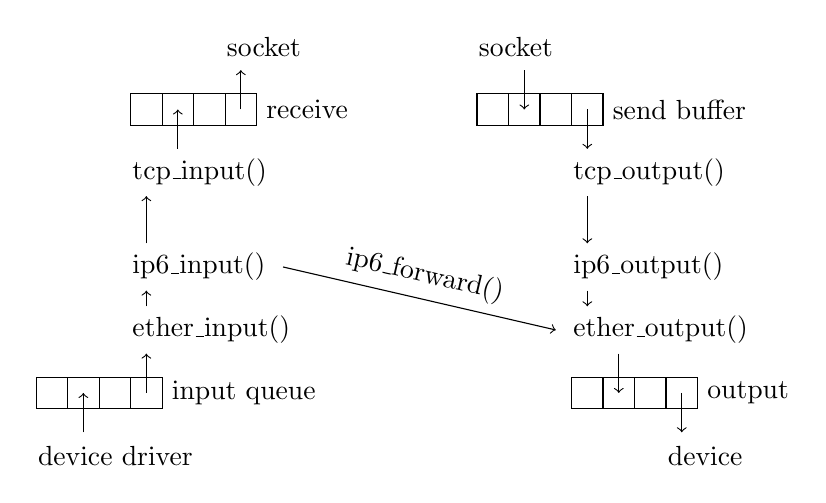
\begin{tikzpicture}
  \draw (0,0)
    node (idd) [right] {device driver} ++(.1,.6)
    rectangle ++(.4,.4) rectangle ++(.4,-.4)
    rectangle ++(.4,.4) rectangle ++(.4,-.4) ++(0,.2)
    node (iq) [right] {input queue} ++(-.5,.8)
    node (ei) [right] {ether\_input()} ++(0,.8)
    node (ii) [right] {ip6\_input()} ++(0,1.2)
    node (ti) [right] {tcp\_input()} ++(.1,.6)
    rectangle ++(.4,.4) rectangle ++(.4,-.4)
    rectangle ++(.4,.4) rectangle ++(.4,-.4) ++(0,.2)
    node (rb) [right] {receive} ++(-.5,.8)
    node (iso) [right] {socket} ++(3.2,0)

    node (oso) [right] {socket} ++(.1,-.6)
    rectangle ++(.4,-.4) rectangle ++(.4,.4)
    rectangle ++(.4,-.4) rectangle ++(.4,.4) ++(0,-.2)
    node (sb) [right] {send buffer} ++(-.5,-.8)
    node (to) [right] {tcp\_output()} ++(0,-1.2)
    node (io) [right] {ip6\_output()} ++(0,-.8)
    node (eo) [right] {ether\_output()} ++(.1,-.6)
    rectangle ++(.4,-.4) rectangle ++(.4,.4)
    rectangle ++(.4,-.4) rectangle ++(.4,.4) ++(0,-.2)
    node (oq) [right] {output} ++(-.5,-.8)
    node (odd) [right] {device}
    ;
  \path (node cs:name=idd,anchor=west) +(.3+1*.4,.3) coordinate (iddo) {};
  \path (node cs:name=iq,anchor=west) +(-.2-2*.4,0) coordinate (iqi) {};
  \draw[->] (iddo) -- (iqi);
  \path (node cs:name=iq,anchor=west) +(-.2,0) coordinate (iqo) {};
  \path (node cs:name=ei,anchor=west) +(.3,-.3) coordinate (iei) {};
  \draw[->] (iqo) -- (iei);
  \path (node cs:name=ei,anchor=west) +(.3,.3) coordinate (eio) {};
  \path (node cs:name=ii,anchor=west) +(.3,-.3) coordinate (iii) {};
  \draw[->] (eio) -- (iii);
  \path (node cs:name=ii,anchor=west) +(.3,.3) coordinate (iio) {};
  \path (node cs:name=ti,anchor=west) +(.3,-.3) coordinate (tii) {};
  \draw[->] (iio) -- (tii);
  \path (node cs:name=ti,anchor=west) +(.3+1*.4,.3) coordinate (iti) {};
  \path (node cs:name=rb,anchor=west) +(-.2-2*.4,0) coordinate (rbi) {};
  \draw[->] (iti) -- (rbi);
  \path (node cs:name=rb,anchor=west) +(-.2,0) coordinate (rbo) {};
  \path (node cs:name=iso,anchor=west) +(.3,-.3) coordinate (isoi) {};
  \draw[->] (rbo) -- (isoi);

  \path (node cs:name=oso,anchor=west) +(.3+1*.4,-.3) coordinate (osoo) {};
  \path (node cs:name=sb,anchor=west) +(-.2-2*.4,0) coordinate (sbi) {};
  \draw[->] (osoo) -- (sbi);
  \path (node cs:name=sb,anchor=west) +(-.2,0) coordinate (sbo) {};
  \path (node cs:name=to,anchor=west) +(.3,.3) coordinate (toi) {};
  \draw[->] (sbo) -- (toi);
  \path (node cs:name=to,anchor=west) +(.3,-.3) coordinate (too) {};
  \path (node cs:name=io,anchor=west) +(.3,.3) coordinate (ioi) {};
  \draw[->] (too) -- (ioi);
  \path (node cs:name=io,anchor=west) +(.3,-.3) coordinate (ioo) {};
  \path (node cs:name=eo,anchor=west) +(.3,.3) coordinate (eoi) {};
  \draw[->] (ioo) -- (eoi);
  \path (node cs:name=eo,anchor=west) +(.3+1*.4,-.3) coordinate (eoo) {};
  \path (node cs:name=oq,anchor=west) +(-.2-2*.4,0) coordinate (oqi) {};
  \draw[->] (eoo) -- (oqi);
  \path (node cs:name=oq,anchor=west) +(-.2,0) coordinate (oqo) {};
  \path (node cs:name=odd,anchor=west) +(.3,.3) coordinate (oddi) {};
  \draw[->] (oqo) -- (oddi);

  \path (node cs:name=ii,anchor=east) +(.1,0) coordinate (ifo) {};
  \path (node cs:name=eo,anchor=west) +(-.1,0) coordinate (ifi) {};
  \draw[->] (ifo) -- (ifi) node [midway,above,sloped] {ip6\_forward()};
\end{tikzpicture}
\end{frame}

\subsection{Netstat Counter}
\begin{frame}[fragile]{Netstat Counter}
netstat -ss
\scriptsize
\begin{verbatim}
ip:
        393285673 total packets received
        246049103 packets for this host
        126364372 packets forwarded
        242653961 packets sent from this host
tcp:
        86520236 packets sent
        123883097 packets received
udp:
        400260722 datagrams received
        82147309 dropped due to full socket buffers
        318113273 delivered
        396391499 datagrams output
ip6:
        434697159 total packets received
        278214439 packets for this host
        146543897 packets forwarded
        240423068 packets sent from this host
\end{verbatim}
\end{frame}

\subsection{pf Test}
\begin{frame}{pf Test}
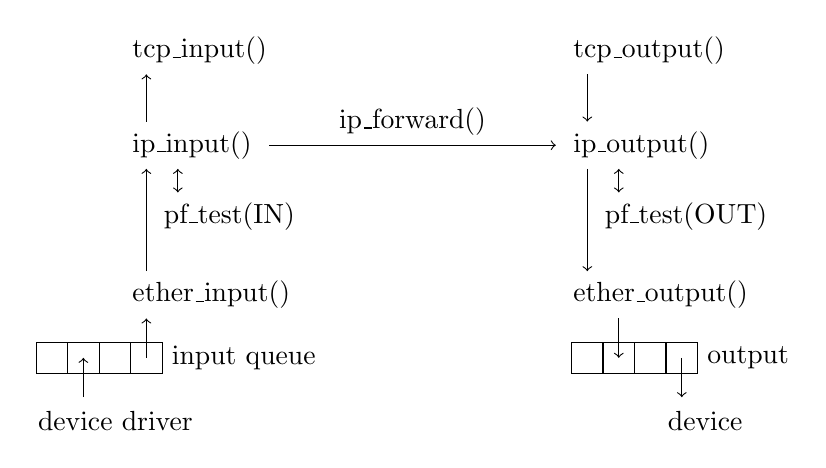
\begin{tikzpicture}
  \draw (0,0)
    node (idd) [right] {device driver} ++(.1,.6)
    rectangle ++(.4,.4) rectangle ++(.4,-.4)
    rectangle ++(.4,.4) rectangle ++(.4,-.4) ++(0,.2)
    node (iq) [right] {input queue} ++(-.5,.8)
    node (ei) [right] {ether\_input()} ++(0.4,1)
    node (pi) [right] {pf\_test(IN)} ++(-0.4,.9)
    node (ii) [right] {ip\_input()} ++(0,1.2)
    node (ti) [right] {tcp\_input()} ++(5.6,0)

    node (to) [right] {tcp\_output()} ++(0,-1.2)
    node (io) [right] {ip\_output()} ++(0.4,-.9)
    node (po) [right] {pf\_test(OUT)} ++(-0.4,-1)
    node (eo) [right] {ether\_output()} ++(.1,-.6)
    rectangle ++(.4,-.4) rectangle ++(.4,.4)
    rectangle ++(.4,-.4) rectangle ++(.4,.4) ++(0,-.2)
    node (oq) [right] {output} ++(-.5,-.8)
    node (odd) [right] {device}
    ;
  \path (node cs:name=idd,anchor=west) +(.3+1*.4,.3) coordinate (iddo) {};
  \path (node cs:name=iq,anchor=west) +(-.2-2*.4,0) coordinate (iqi) {};
  \draw[->] (iddo) -- (iqi);
  \path (node cs:name=iq,anchor=west) +(-.2,0) coordinate (iqo) {};
  \path (node cs:name=ei,anchor=west) +(.3,-.3) coordinate (iei) {};
  \draw[->] (iqo) -- (iei);
  \path (node cs:name=ei,anchor=west) +(.3,.3) coordinate (eio) {};
  \path (node cs:name=ii,anchor=west) +(.3,-.3) coordinate (iii) {};
  \draw[->] (eio) -- (iii);
  \path (node cs:name=ii,anchor=west) +(.3,.3) coordinate (iio) {};
  \path (node cs:name=ti,anchor=west) +(.3,-.3) coordinate (tii) {};
  \draw[->] (iio) -- (tii);
  \path (node cs:name=ii,anchor=west) +(.7,-.3) coordinate (iip) {};
  \path (node cs:name=pi,anchor=west) +(.3,.3) coordinate (pii) {};
  \draw[<->] (iip) -- (pii);

  \path (node cs:name=to,anchor=west) +(.3,-.3) coordinate (too) {};
  \path (node cs:name=io,anchor=west) +(.3,.3) coordinate (ioi) {};
  \draw[->] (too) -- (ioi);
  \path (node cs:name=io,anchor=west) +(.3,-.3) coordinate (ioo) {};
  \path (node cs:name=eo,anchor=west) +(.3,.3) coordinate (eoi) {};
  \draw[->] (ioo) -- (eoi);
  \path (node cs:name=eo,anchor=west) +(.3+1*.4,-.3) coordinate (eoo) {};
  \path (node cs:name=oq,anchor=west) +(-.2-2*.4,0) coordinate (oqi) {};
  \draw[->] (eoo) -- (oqi);
  \path (node cs:name=oq,anchor=west) +(-.2,0) coordinate (oqo) {};
  \path (node cs:name=odd,anchor=west) +(.3,.3) coordinate (oddi) {};
  \draw[->] (oqo) -- (oddi);
  \path (node cs:name=io,anchor=west) +(.7,-.3) coordinate (iop) {};
  \path (node cs:name=po,anchor=west) +(.3,.3) coordinate (poi) {};
  \draw[<->] (iop) -- (poi);

  \path (node cs:name=ii,anchor=east) +(.1,0) coordinate (ifo) {};
  \path (node cs:name=io,anchor=west) +(-.1,0) coordinate (ifi) {};
  \draw[->] (ifo) -- (ifi) node [midway,above] {ip\_forward()};
\end{tikzpicture}
\end{frame}

\subsection{Patches for TCP Input}
\begin{frame}{Patches for TCP Input}
    \begin{adjustbox}{totalheight=\textheight-3\baselineskip}
        \input{gnuplot/2025-01-26T17-08-00Z-tcp-0,1,2,3.tex}
    \end{adjustbox}
\end{frame}

\subsection{Parallel TCP Receive}
\begin{frame}{Parallel TCP Receive}
    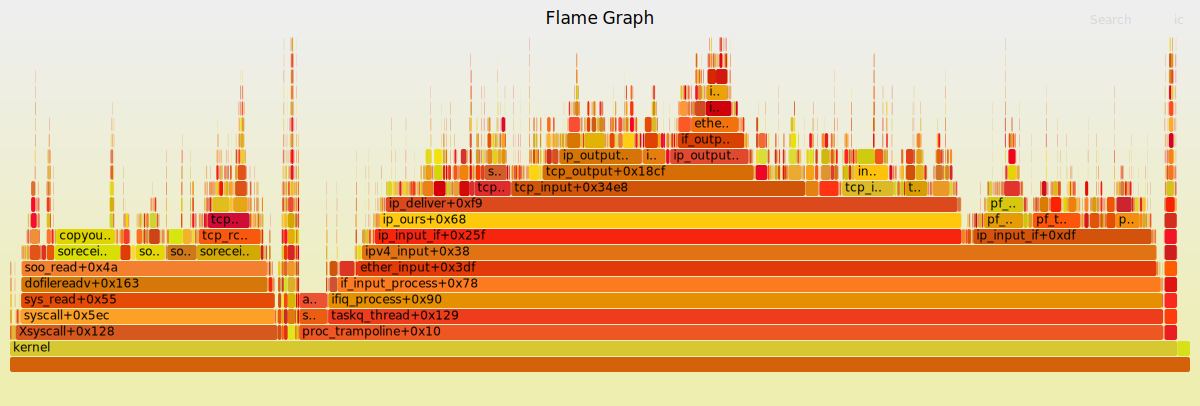
\includegraphics[width=\textwidth]{kstack/sys-tcp-mpinput-rev-parallel.pdf}
\end{frame}

\end{document}
